\subsection{Exploratory Visualization}
A visualization has been provided that summarizes or extracts a relevant characteristic or feature about the dataset or input data with thorough discussion. Visual cues are clearly defined.


There are 60,000 of images in total. Figure(50,000 images for training data and 10,000 images for test data).\ref{fig:two} shows the samples of the images. I plotted 10 images for each class.Figure.\ref{fig:three} and Figure.\ref{fig:four} shows the distribution of the data. For the training dataset, each class has 5,000 images and for the test dataset, each class has 1,000 images.
The label 0 to 9 corresponds to 'Airplane','Automobile','Bird','Cat','Deer','Dog','Frog','Horse','Ship, and 'Truck'.
\begin{figure}[htbp]

\begin{center}
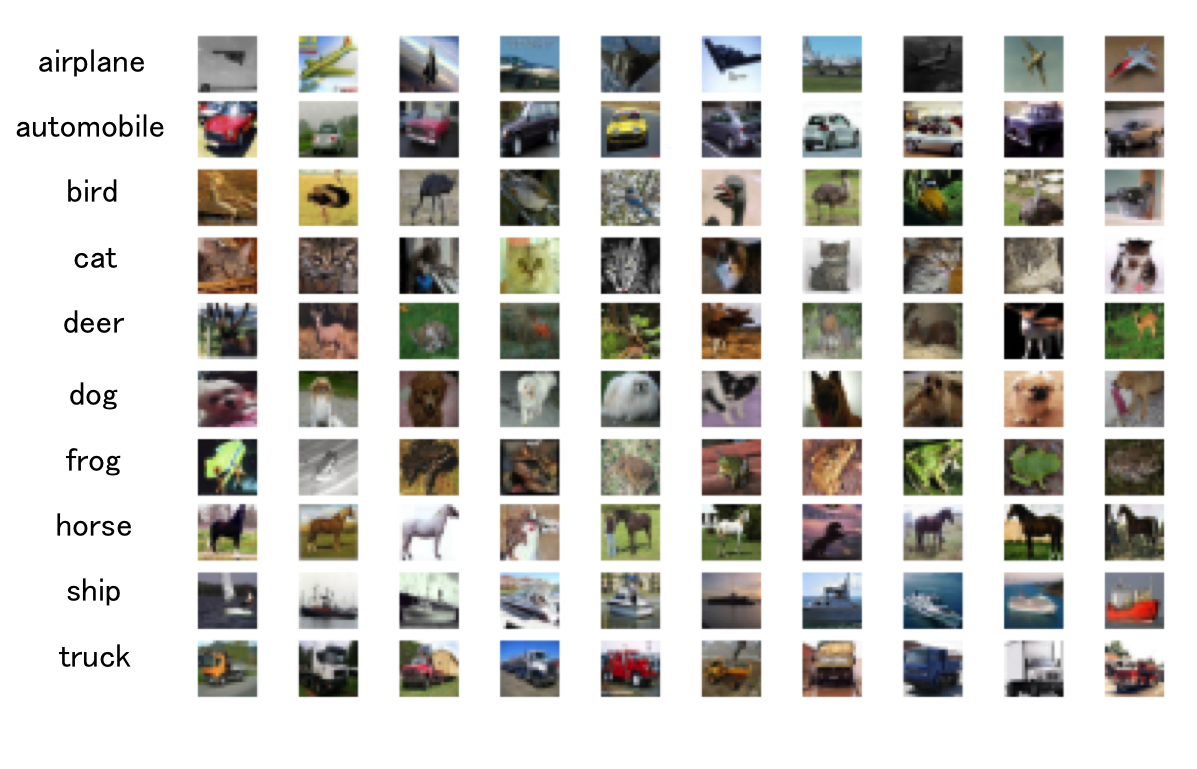
\includegraphics[width=10cm]{picture/random_sample.png}
\end{center}
\caption{Sample of the Images}
\label{fig:two}

\end{figure}

\begin{figure}[h]
\begin{minipage}{0.5\hsize}
	\begin{center}
	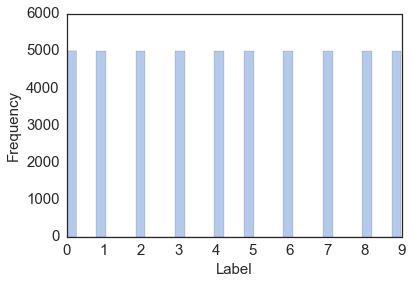
\includegraphics[width=5cm]{picture/Distribution_of_Training_Data.png}
	\end{center}
	\caption{Distribution of Training Data}
	\label{fig:three}
\end{minipage}
\begin{minipage}{0.5\hsize}
\begin{center}
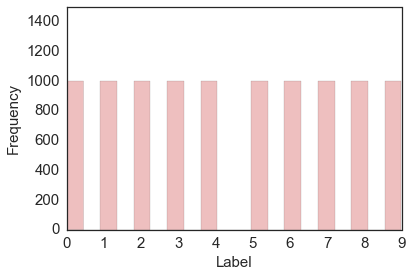
\includegraphics[width=5cm]{picture/Distribution_of_Test_Data.png}
\end{center}
 \caption{Distribution of Test Data}
  \label{fig:four}
 \end{minipage}
\end{figure}

